%!TEX root = ../main.tex

\section{Efficient Global Optimization}\label{sec:}

We now have two options for convex optimization of ReLU models: directly tackling the C-ReLU problem or solving C-GReLU and a cone decomposition program (see \cref{fig:relations}).
This section develops efficient and scalable methods for both approaches.
For simplicity, we assume \(\mathcal{L}\) is squared loss; our results are easily extended to other loss functions.

\subsection{Solving the Gated ReLU Problem}\label{sec:r-fista}

Our goal is a fast and reliable method for the C-GReLU problem even when \( \tilde \calD \) is very large.
To be practical, it should benefit from GPU acceleration, provide convergence certificates, and be ``tuning-free''.
To be theoretically satisfying, it should come with complexity guarantees.

Our starting place is the observation that C-GReLU is exactly the classic \emph{group lasso} with basis expansion,
\[ M(X) = [D_1 X \, D_2 X \, \cdots \, D_{\abs{\tilde \calD}} X ]. \]
A naive approach to huge-scale group lasso is the stochastic subgradient method;
this approach benefits from auto-differentiation engines such as PyTorch~\citep{paszke2019pytorch} and TensorFlow~\citep{abadi2016tensorflow} and is simple to code.
However, subgradient methods require decreasing step-sizes to converge and are extremely slow --- they require \( O(\epsilon^{-2}) \) iterations to to compute an \( \epsilon \)-optimal point.

Instead, we use the composite structure of the objective as a sum of a convex quadratic \( f(u) = \|\sum_{D_i \in \tilde \calD} D_i X u_i - y\|_2^2 \) and the non-smooth penalty \( g(u) = \lambda \sum_{D_i \in \tilde \calD} \norm{u_i}_2 \).
The FISTA algorithm~\citep{beck2009fista} is an accelerated method that treats \( g \) exactly using the iteration,
\begin{align}
    \xkk
     & = \argmin_{y} Q_{\yk, \etak}(y) + g(y)               \label{eq:prox-gradient-mm} \\
    \ykk
     & = \xkk + \frac{t_k - 1}{t_{k + 1}} \rbr{\xkk - \xk} \nonumber,
\end{align}
where \( t_{k + 1} = (1 + \sqrt{1 + 4 t_k^2}) / 2 \, \) and,
\begin{equation*}
    \begin{aligned}
        Q_{\xk, \etak}(y) & = f(\xk)  +  \abr{\grad(\xk), y  -  \xk}
        +  \frac{1}{2 \etak}\norm{y  -  \xk}_2^2,
    \end{aligned}
\end{equation*}
majorizes \( f \) as long as \( \etak \leq \lambda_{\text{max}}(M^\top M)^{-1} \).
Using the convergence guarantee for FISTA when \( f, g \) are convex and $f$ is Lipschitz smooth~\citep{duchi2009forwardbackwardsplitting, beck2009fista, nesterov2007proximalgradient} gives the complexity of \emph{global} optimization of the NC-GReLU problem.

\begin{restatable}{theorem}{gatedComplexity}\label{thm:gated-complexity}
    Let \( \theta^* = \rbr{W^{*(1)}, W^{*(2)}} \) be the minimum-norm global
    minimizer of the NC-GReLU problem with gates \( \calG \).
    Then, we can compute an \( \epsilon \)-optimal point
    \( \theta_\epsilon = (\rbr{W^{(1)}_\epsilon, W^{(2)}_\epsilon}) \) in
    iterations
    \begin{equation*}
        \begin{aligned}
            T & \leq \big(2 \epsilon^{-1} \lambda_{\text{max}}\rbr{M^\top
                M}\sum_{D_i \in \tilde \calD} \norm{W^{*(1)}_{\cdot, i}
                W^{*(2)}_{i}}_2^2\big)^{1/2}.
        \end{aligned}
    \end{equation*}
\end{restatable}

Proof in \cref{app:optimization}.
\cref{thm:gated-complexity} can also be expressed directly in terms of the C-GReLU problem by using a mapping between minimizers of the convex and non-convex formulations.
Data normalization gives \( \lambda_{\text{max}}\rbr{M^\top M} \leq d \cdot |\tilde \calD |  \), which is fully polynomial when \( \text{rank} (X) \) is constant (see Appendix~\ref{app:data-normalization}).
Such a condition holds for convolutional networks with fixed filter sizes~\citep{pilanci2020convexnn}.

\subsubsection{Developing an Efficient Optimizer}\label{sec:efficient-fista}

In theory, it is sufficient to run FISTA with small enough step-size to obtain \cref{thm:gated-complexity}, but this approach works poorly in practice.
Additional enhancements are required for fast and reliable solvers.

\textbf{Line-Search}:
Constant step-sizes converge slowly, so we use a line-search with the test condition proposed by \citet{beck2009fista}:
\begin{equation}\label{unconstrained:eq:line-search-cond}
    f(\xkk(\etak)) \leq Q_{\yk, \etak}(\xkk(\etak)).
\end{equation}
Computing this condition requires evaluating \( f(\xkk(\etak)) \), but does not need additional gradient evaluations like the alternative proposed by~\citet{nesterov2007proximalgradient}.
%Sadly, unlike the Armijo condition~\citep{armijo1966ls}, \cref{unconstrained:eq:line-search-cond} does not guarantee decrease on $F$ or $f$.
Simple backtracking along \( \xkk - \xk \)  works poorly and does not converge;
instead, we probe the arc of solutions to~\eqref{eq:prox-gradient-mm} by reducing the step-size.
As evaluating the proximal operator is slower than backtracking, it is important to initialize \( \etak \) effectively.

\textbf{Initializing the Step-size}:
Warm-starting with \( \etak = \eta_{k-1} \) can lead to overly-small steps, particularly later in optimization.
An alternative is \emph{forward-tracking} as \( \eta_k = \alpha \eta_{k-1} \) for \( \alpha > 1 \) \citep{fridovich2019choosing}.
This can partially adapt to local Lipschitz smoothness of \( f \), but may also lead to unnecessary evaluations of the proximal operator.
Instead, we check the tightness of~\eqref{unconstrained:eq:line-search-cond} before forward-tracking~\citep{liu2009lassplore}.
Let \( l_{\yk}(\x) = f(\yk) + \abr{\grad(\yk), \x - \yk} \) and
\begin{equation}\label{unconstrained:eq:upper-bound-gap}
    \omega_k := \frac{\norm{\xk - \y_{k-1}}_2^2}{2 \eta_{k-1} \rbr{f(\xk) - l_{\y_{k-1}}(\xk)}},
\end{equation}
to get \( \eta_{k} = \eta_{k-1} + (1 - \alpha) \eta_{k-1} \mathds{1}(\omega_k \geq c)\);
\( c = 1 \) obtains forward-tracking, while \( c \gg 1 \) gives a conservative strategy.

\textbf{Restarts}:
Resetting \( (\yk, t_k) \gets (\xk, 1) \) in the middle of optimization is called \emph{restarting}.
Restarting methods adapt to strong convexity and can attain a fast linear rate of convergence~\citep{nesterov2007proximalgradient, allen2014linear}.
Although C-GReLU is not strongly-convex, restarts can allow FISTA to adapt to local curvature~\citep{giselsson2014restart}.
We restart FISTA when
\( \abr{\xkk - \xk, \xkk - \yk} > 0 \) --- that is, \( \xkk \) is not a descent step with respect to the proximal gradient mapping~\citep{odonoghue2015restarts}.

\textbf{Data Normalization}: The proximal step~\eqref{unconstrained:eq:line-search-cond} is equivalent to composition of a gradient update with the group soft-thresholding operator.
Thresholding is sensitive to rounding errors in computation of the gradient and,
since errors accumulate in the ``memory'' \( y_k \), it is critical to improve
the conditioning of this computation.
Appendix~\ref{app:data-normalization} describes a simple data transformation which works well in practice.

Combining these elements together gives an efficient algorithm for C-GReLU which we call R-FISTA.
%(Algorithm~\ref{alg:r-fista}).

%% accelerated proximal gradient algorithm w/ line-search %%
%\setlength{\algomargin}{1em}
%\begin{algorithm}[t]
%    \SetAlgoLined
%    \KwIn{\( f, g, \x_0, \eta_0, c, \beta, \alpha \)}
%    \( t_0 \gets 1, \y_0 \gets \x_0 \)\;
%    \For{\(k = 0 \ldots K - 1\)}{
%        \( \xkk \gets \argmin_{y} Q_{yk, \etak}(y) \)\;
%        \While{\( f(\xkk(\etak)) > Q_{\yk, \etak} \)}{
%            \( \etak \gets \etak \cdot \etak \)\;
%            \( \xkk \gets \argmin_{y} Q_{yk, \etak}(y) \)\;
%        }
%        \( t_{k + 1} \gets \frac{1 + \sqrt{1 + 4 t_k^2}}{2} \) \;
%        \( \ykk \gets \xkk + \frac{t_k - 1}{t_{k + 1}} \rbr{ \xkk - \xk} \) \;
%        \If{\( \abr{\xkk - \xk, \xkk - \yk} > 0 \)}{
%            \( t_{k + 1} \gets 1 \), \( \ykk \gets \xkk \) \;
%        }
%        \( \omega_{k+1} \gets \frac{\norm{\xkk - \yk}_2^2}{\etak \sbr{f(\xkk) - l_{\yk}(\xkk)}} \) \;
%        \( \etakk \gets \etak  + (\alpha - 1) \etak \mathds{1}(\omega_{k+1} \geq c) \) \;
%    }
%    \Return{\( \x_{K-1} \)}
%    %%
%    \caption{R-FISTA.}%
%    \label{alg:r-fista}
%\end{algorithm}

\subsection{Tractable Cone Decompositions}\label{sec:cone-decomp}

Training a ReLU network using \cref{alg:cone-decomp} requires solving a large-scale LP or SOCP.
Empirically, the complexity of solving these problems with commercial software is similar to directly solving C-ReLU (see \cref{table:cone-decomp}).
Instead, we propose an \emph{approximate} decomposition procedure which
can be solved efficiently using R-FISTA.

Manipulating the cone decomposition \( v - w = u \), \( v, w \in \calK \),
we obtain the equivalent conditions \( \tilde X w \geq (-\tilde X u)_+ \) and \( v = u + w \).
Given
\( \rho \geq 0 \), and \( b = (-\tilde X u)_+ \),
the regularized one-sided quadratic
\begin{equation}\label{eq:cd-approx}
    \textbf{CD-A}: \, \min_{w} \half
    \|
    (b - \tilde X w)_+
    \|_2^2
    + \rho \norm{w}_2,
\end{equation}
approximates the exact cone-decomposition as follows:
\begin{restatable}{proposition}{approxDecompBounds}\label{prop:approx-decomp-bounds}
    Suppose \( \tilde w \) is a minimizer of \eqref{eq:cd-approx} and let \( \tilde v = u + \tilde w \).
    If \( X \) is full row-rank, then
    \[
        \|(\tilde X \tilde w)_-\|_2 + \|(\tilde X \tilde v)_-\|_2
        \leq \frac{2\rho}{\sigma_{\text{min}}(\tilde X)}.
    \]
    Furthermore, if \( \rho > 0 \), then the norm bound in \cref{prop:socp-decomp} also holds for the approximate solution \( (\tilde v, \tilde w) \).

    Alternatively, suppose \( X \) is not full row-rank.
    As \( \rho_k \rightarrow 0 \), every convergent subsequence of \( (\tilde v_k, \tilde w_k) \) is a feasible cone decomposition.
    Moreover, at least one such sequence exists.
\end{restatable}
Proof in \cref{app:optimization}, where we also provide \cref{prop:approx-decomp-submatrices},
an alternative characterization in terms of sub-matrices \( \tilde X_{\calJ} \).
\autoref{prop:approx-decomp-bounds} shows it is straightforward to control the quality of the approximation by tuning \( \rho \).
In practice, we find CD-A with \( \rho \approx 10^{-10} \) yields competitive performance and is easily solved using R-FISTA.

\subsection{Solving the ReLU Problem}\label{sec:al-method}

The main difficulty in solving C-ReLU is the constraints.
%Projecting onto \( \calK_i \) is a quadratic program, making proximal-gradient methods unfeasible.
Interior point methods~\citep{nesterov1994interior} and specialized conic solvers~\citep{odonoghue2016scs} can handle \( \calK_i \), but such methods require second-order information or repeated linear-system solves and scale poorly in both \( n \) and \( d \).
Instead, we develop an augmented Lagrangian (AL) method that uses R-FISTA as a sub-routine.

Recall \cref{thm:cone-elimination} established a sub-sampled problem equivalent to the full C-ReLU problem for which each \( \calK_i \) is non-singular.
These cones have an interior point if and only if they are non-singular (see \cref{lemma:affine-characterization}), implying the sub-sampled problem is strictly feasible and satisfies strong duality.
Letting \( \gamma, \zeta \in \R^{|\tilde \calD| \times n} \) be estimates of the optimal Lagrange multipliers, the augmented Lagrangian for~\eqref{convex-forms:eq:convex-relu-mlp} is
\begin{equation}\label{eq:augmented-lagrangian}
    \begin{aligned}
        \calL_\delta & (v, w, \gamma, \zeta) := (\delta / 2)  \sum_{D_i \in \tilde \calD}  \big[\|(\gamma_i / \delta -  \tilde X_i v_i)_+\|_2^2 \\
                     & \hspace{2em} + \|(\zeta_i / \delta - \tilde X_i w_i)_+\|_2^2 \big] + F(v,w),
    \end{aligned}
\end{equation}
where \( F(v, w) \) is the primal objective and \( \tilde X_i = (2 D_i - I) X \).
Eq.~\ref{eq:augmented-lagrangian} is a penalty method and can recover an optimal primal-dual pair from \( \rbr{v_k, w_k} \in \argmin \calL_{\delta_k}(v, w, 0, 0) \) as \( \delta_k \into \infty \) \citep{nocedal1999numerical}.
However, choosing \( \delta_k \) is challenging in practice.

\begin{figure*}[t]
    \centering
    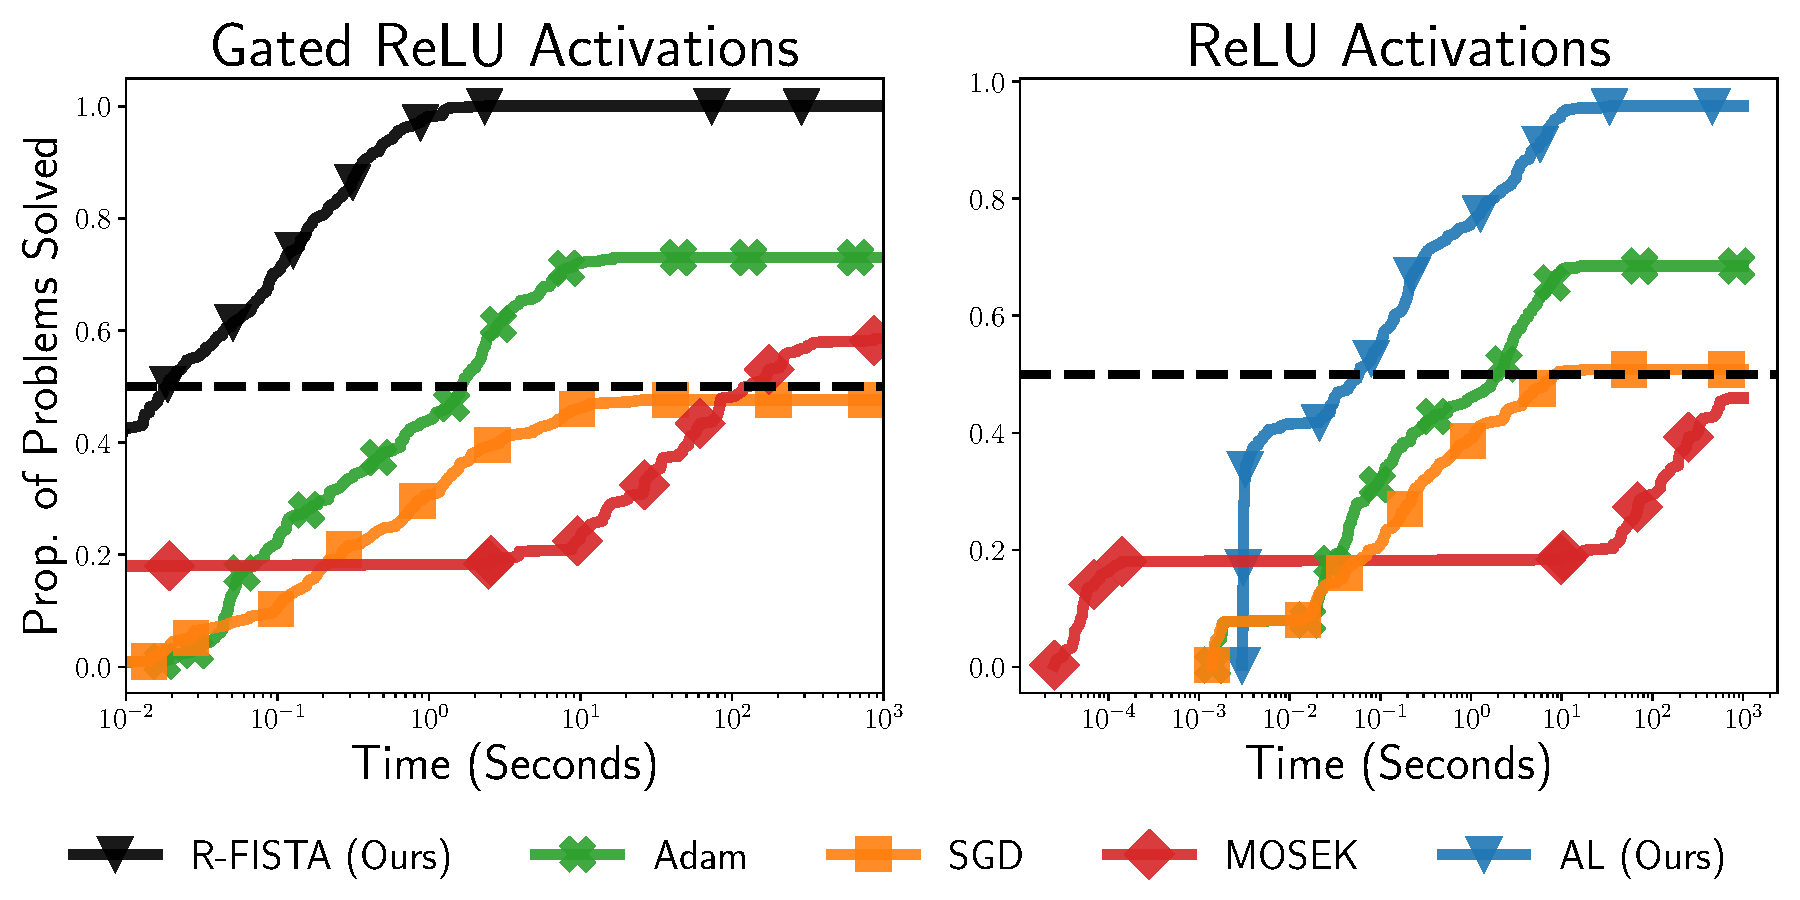
\includegraphics[width=0.9\linewidth]{figures/chapter_two/pp_main.pdf}
    \vspace{-0.4cm}
    \caption{Performance profiles comparing (left) R-FISTA and MOSEK for the C-GReLU problem to Adam and SGD for NC-GReLU,
        and (right) the AL method and baselines for C-ReLU/NC-ReLU.
        A problem is solved when \( \rbr{F(x_k) - F(x^*)}/F(x^*) \leq 1 \), where \( F(x^*) \) is the smallest objective value found by any method.
        This rule is method-independent as the convex and non-convex problems share the same optimal objective value.
        See Appendix~\ref{app:performance-profiles} for alternative thresholds.
        Methods are judged by comparing time to a fixed proportion of problems solved (see dashed line at \( 50\% \)).
        R-FISTA and the AL method solve a higher proportion of problems faster than the baselines.
    }%
    \label{fig:performance-profiles}
    \vspace{-0.4cm}
\end{figure*}

Instead, the AL method performs proximal-point iterations on the dual \citep{rockafellar1976monotone, rockafellar1976augmented} via the iterations,
\begin{align}
    \rbr{v_{k+1}, w_{k+1}}
                & = \argmin_{v, w} \calL_{\delta}(v, w, \gamma_k, \zeta_k), \label{eq:al-subroutine} \\
    \gamma_{k + 1}
    = (\gamma_k & - \delta \tilde X_i v_i)_+, \quad
    \zeta_{k + 1} = (\zeta_k - \delta \tilde X_i w_i)_+. \nonumber
\end{align}
The dual iterates of the AL method converge as \( O(1/\delta \cdot \epsilon) \). See \cref{thm:al-convergence-rate} for a proof going through proximal-point.

\subsubsection{Reliable Constrained Optimization}\label{sec:reliable-co}

AL methods are typically \emph{exterior point} solvers: \( (v_k, w_k) \) will approach the constraint set only as the dual problem is solved.
The complexity of maximizing the dual depends on the penalty strength, with \( \delta \gg 1 \) producing fast convergence.
However, \( \delta \) also affects the Lipschitz smoothness of \( \calL_\delta \) --- large \( \delta \) increases the curvature of the (one-sided) quadratic penalties --- and can make solving~\eqref{eq:al-subroutine} prohibitively expensive for first-order methods.
Thus, we choose \( \delta \) to balance convergence on the primal and dual problems.

\textbf{Choosing the Penalty Strength}:
it is common to set \( \delta \) to aggressively decrease the constraint gap~\citep{conn2013lancelot, murtagh1983minos},
\[ c_{\text{gap}} = \sum_{D_i \in \tilde \calD} \|(\tilde X_i v_i)_-|^2_2 + \|(\tilde X_i w_i)_-\|^2_2. \]
These rules pre-suppose second-order solvers and lead to very poor conditioning of \( \calL_\delta \).
Instead, we propose a simple ``windowing'' heuristic:
when solving Eq.~\ref{eq:al-subroutine} for \( \rbr{\gamma_1, \zeta_1} \), take \( \delta \) to ensure that \( c_{\text{gap}} \in \sbr{r_{\text{l}}, r_{\text{u}}} \).
This condition can be checked and enforced with minimal overhead by using a mild convergence criterion initially and helps avoid extreme behavior.
We found \( [r_{\text{l}}, r_{\text{u}}] = [0.01, 0.1] \) works well.

\textbf{Warm Starts}: The contours of \( \calL_\delta\rbr{\cdot, \cdot, \gamma_{k+1}, \zeta_{k+1}} \) typically change slowly when \( \delta \) is moderate.
In such cases, minimizing the augmented Lagrangian can be greatly sped-up by warm-starting with \( \rbr{v_k, w_k} \).

We obtain an efficient and robust AL method by combining warm-starts, our heuristic for \( \delta \), and the R-FISTA sub-solver.

